% alg-p2-05: 完全平方公式几何拼图
% (a+b)^2 = a^2 + 2ab + b^2
% 大正方形边长 a+b，分为四块：a×a, a×b, b×a, b×b
\documentclass[tikz,border=4pt]{standalone}
\usepackage{ctex}
\usepackage{amsmath}
\usetikzlibrary{calc}
\begin{document}
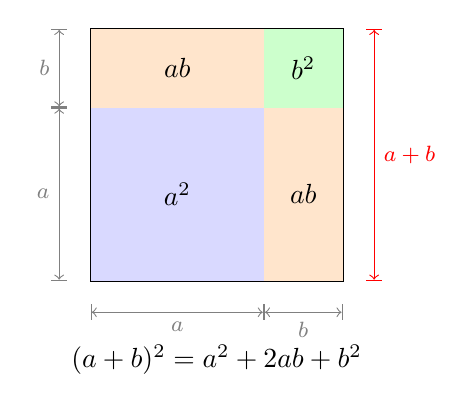
\begin{tikzpicture}[scale=1.0, thick]

  % 参数：a=2.2, b=1.0（用于绘图比例）
  \pgfmathsetmacro{\a}{2.2}
  \pgfmathsetmacro{\b}{1.0}
  \pgfmathsetmacro{\ab}{\a+\b}

  % 大正方形外框
  \draw[thick] (0,0) rectangle (\ab,\ab);

  % 内部分割线
  \draw[thick] (\a,0) -- (\a,\ab);   % 竖线，分 a | b
  \draw[thick] (0,\a) -- (\ab,\a);   % 横线，分 a | b（从下往上）

  % ---- 各块填色与标注 ----

  % 左下：a×a（蓝色浅填）
  \fill[blue!15] (0,0) rectangle (\a,\a);
  \node at (\a/2, \a/2) {$a^2$};

  % 右下：b×a（橙色浅填，即 ab）
  \fill[orange!20] (\a,0) rectangle (\ab,\a);
  \node at (\a+\b/2, \a/2) {$ab$};

  % 左上：a×b（橙色浅填，即 ab）
  \fill[orange!20] (0,\a) rectangle (\a,\ab);
  \node at (\a/2, \a+\b/2) {$ab$};

  % 右上：b×b（绿色浅填）
  \fill[green!20] (\a,\a) rectangle (\ab,\ab);
  \node at (\a+\b/2, \a+\b/2) {$b^2$};

  % ---- 边长标注 ----
  % 下边：a 和 b
  \draw[|<->|, thin, gray] (0,-0.4) -- node[below, font=\footnotesize] {$a$} (\a,-0.4);
  \draw[|<->|, thin, gray] (\a,-0.4) -- node[below, font=\footnotesize] {$b$} (\ab,-0.4);

  % 左边：a 和 b
  \draw[|<->|, thin, gray] (-0.4,0) -- node[left, font=\footnotesize] {$a$} (-0.4,\a);
  \draw[|<->|, thin, gray] (-0.4,\a) -- node[left, font=\footnotesize] {$b$} (-0.4,\ab);

  % 大正方形边长（右边）
  \draw[|<->|, thin, red] (\ab+0.4,0) -- node[right, font=\footnotesize, red] {$a+b$} (\ab+0.4,\ab);

  % 公式标注
  \node[font=\normalsize] at (\ab/2, -1.0)
    {$(a+b)^2 = a^2 + 2ab + b^2$};

\end{tikzpicture}
\end{document}
